\documentclass[10pt, a4paper]{article} % Abbassato a 11pt per bilanciare l'interlinea doppia di LaTeX

% Pacchetti base
\usepackage[utf8]{inputenc}
\usepackage[english]{babel}
\usepackage{blindtext} 
\usepackage{cite} 
\usepackage{natbib}
\usepackage{amsmath}
\usepackage{booktabs} 
\usepackage{pgfplots}
\usepackage{rotating}   % nel preambolo, al posto di pdflscape
\usepackage{booktabs}
\usepackage{threeparttable}
\usepgfplotslibrary{groupplots}
% Margini APA (1 pollice)
\usepackage{geometry}
\geometry{a4paper, margin=1in}

% Spaziatura APA
\usepackage{setspace}
\doublespacing

% Paragrafi APA (niente spazi extra, solo rientro)
\setlength{\parskip}{0pt}
\setlength{\parindent}{0.5in}
% Informazioni sul documento

\title{\textbf{Opening the Black Box:} \\ 
\textbf{XAI and Algorithm Aversion in Bear Markets}}

\author{Gabriele Matteo Antonini \\ \textit{EBS Universität für Wirtschaft und Recht} \\ \textit{Fundamentals of Experimental Design and Analysis}}
\date{July 2026}

\begin{document}

\maketitle

\begin{abstract}
\noindent Financial firms are increasingly relying on machine learning models and automated algorithms. However, many investment funds do not explicitly advertise their use of AI, possibly to avoid reputational repercussions stemming from general public skepticism.
While investors' reluctance to rely on automated strategies, often termed algorithm aversion, is well documented \citep{dietvorst2015algorithm}, this paper investigates whether this aversion is driven by a lack of understanding and can thus be mitigated by Explainable AI (XAI). Furthermore, it explores how this dynamic interacts with market contexts, hypothesizing that the need for XAI is more pronounced during market downturns (bear markets) and among investors with lower financial literacy.
To test these hypotheses, this preliminary study employed a 2 $\times$ 2 $\times$ 2 factorial design, analyzing the simulated responses of a synthetic sample of 100 Digital Twins via Large Language Models (LLMs), through a robust analytical approach (non-parametric Aligned Rank Transform ANOVA).
The results revealed a significant three-way interaction between market context, algorithmic transparency, and financial literacy. 
Specifically, XAI significantly mitigated algorithm aversion during bear markets, but exclusively for individuals with low financial literacy; conversely, in bull markets, XAI generated a significant trust premium primarily among highly literate investors, suggesting a more complex pattern than initially hypothesized.
These findings highlight the context-dependent nature of algorithmic trust and suggest that investment funds could benefit from tailoring transparency strategies to specific investor segments and market conditions, rather than adopting a uniform disclosure approach, in order to reduce customer churn and foster trust across market cycles.
\end{abstract}

\newpage

\section{Introduction}

The financial industry is currently experiencing a profound technological paradigm shift, increasingly relying on artificial intelligence (AI) and machine learning models to automate data analysis, investment decisions, and trade execution, ranging from high-frequency trading to retail robo-advisors. However, a distinct paradox has emerged in recent years: despite the widespread adoption of these technologies, numerous investment funds avoid explicitly advertising their use of AI to retail clients \citep{esma2023artificial}. This opacity is likely a strategic choice to avoid trust erosion and prevent customer churn.

The root of this reputational risk lies in the well-documented phenomenon of algorithm aversion \citep{dietvorst2015algorithm}, characterized by individuals' persistent skepticism toward automated systems even when these outperform human judgment. In the financial domain, this translates into investor reluctance to trust automated strategies. The prior body of work, however, leaves a critical gap: while recent research indicates that Explainable AI (XAI) - methods providing clear interpretation of AI algorithms - can significantly enhance transparency and decision-making trust in financial services \citep{Staley2025TheRole}, previous studies have largely treated algorithm aversion as a static trait, failing to account for how it dynamically fluctuates across market contexts and the emotional and cognitive responses these contexts trigger in individuals with different levels of financial literacy. Emerging evidence further suggests that emotions mediate investors' responses to AI disclosure \citep{Downen2024Algorithm}, though this mechanism has not yet been rigorously tested across diverse market contexts and literacy profiles.

To bridge this gap, I address the following research question: \textit{Does Explainable AI (XAI) reduce investor algorithm aversion, and if so, how do market contexts (bull vs.\ bear) and individual financial literacy levels jointly moderate this effect?} By addressing this, my study shifts the academic discourse from a generalized view of algorithmic trust toward a contingency-based framework. I hypothesize that XAI serves as a critical mechanism for increasing willingness to invest, an effect notably amplified among individuals with lower financial literacy who rely on the XAI-provided rationale as essential `analytical scaffolding' to rationalize financial risk \textit{(Hypothesis 1)}. This is consistent with the broader principle that the psychological need for transparency intensifies precisely when outcomes are uncertain and difficult to independently verify. In addition, I argue that this mitigation effect is dependent on the market context, expecting the positive influence of XAI to be more pronounced during bear markets, where uncertainty and fear heighten the need for trust. Conversely, I explore whether market euphoria, often associated with momentum and FOMO, acts as a buffer that attenuates the demand for explainability among highly literate profiles, effectively overriding the psychological requirement for transparency \textit{(Hypothesis 2)}. This matters beyond theory: clarifying \textit{when} algorithm aversion peaks, and for whom, allows investment funds to move from a costly blanket transparency strategy toward a targeted deployment of explainability features, reducing client attrition without unnecessary implementation costs.

Methodologically, this preliminary analysis leverages an innovative computational approach. Rather than relying on a traditional survey, this study employs Large Language Models (LLMs) to instantiate a synthetic sample of 100 \textit{Digital Twins}. By utilizing real socio-demographic profiles to perform \textit{persona-prompting} via API, the LLM simulates human-like cognitive biases and financial decision-making processes, offering a highly scalable and controlled experimental environment.

The preliminary results partially confirm the hypotheses, revealing a significant three-way interaction between market context, algorithmic transparency, and financial literacy.

\section{Experimental Design and Methodology}

\subsection{Experimental Design and Variables}

In this preliminary investigation, the study employs a $2 \times 2 \times 2$ between-subjects factorial design, analyzed via the non-parametric Aligned Rank Transform (ART) ANOVA \citep{wobbrock2011thealigned}. \footnote{The ART ANOVA was preferred over a traditional parametric ANOVA because the latter relies on a strong normality assumption for the dependent variable, which is unlikely to hold for an ordinal 1-7 Likert scale. This was confirmed via a Kolmogorov-Smirnov test against a normal distribution with matched mean and standard deviation ($D = 0.329$, $p < .001$), indicating a significant departure from normality and justifying the non-parametric approach. Moreover, the proposed method is robust to unbalanced designs.}\footnote{Since the Kolmogorov-Smirnov test assumes a continuous distribution; given the discrete nature of the 1-7 Likert scale, this result should be interpreted as indicative rather than exact, though it is consistent with the visibly non-normal distribution of the raw data.} The adoption of a factorial, variance-based approach to test the moderating effects of algorithmic transparency on investment intentions is strongly consistent with recent experimental paradigms in behavioral finance \citep{chang2026does}. The design comprises the following elements:
\begin{itemize}
    \item \textbf{Dependent Variable:} Willingness to Invest (measured on a continuous 1-7 Likert scale, where 1 indicates ``Absolutely not willing to invest'' and 7 indicates ``Extremely willing to invest'').
    \item \textbf{Independent Variables:} 
    \begin{itemize}
        \item \textit{Market Context:} Bull Market (described as a thriving economy with consistent growth and high consumer confidence) vs. Bear Market (described as a severe downturn characterized by high volatility and significant uncertainty).
        \item \textit{Algorithmic Transparency:} Standard AI (opaque/black-box, described as providing only standard performance KPIs with ``proprietary and completely hidden'' internal logic) vs. Explainable AI (XAI, described as providing a dashboard showing ``exact decision rationales, feature weights, and risk assessments'').
        \item \textit{Financial Literacy:} Categorized as High vs. Low based on a median split of the individual's baseline score, serving as a core moderator of algorithmic trust.
    \end{itemize}
\end{itemize}

Note: While technological knowledge (Tech Savviness) was initially considered as a potential covariate, it was excluded from the final model to prevent multicollinearity, given its high correlation with financial literacy.

Future iterations of this research intend to expand this preliminary framework using an Aligned Rank Transform procedure for covariates, which will retain financial literacy in its continuous form and systematically control for a broader set of demographic and psychological covariates. These could include age, income, gender, and average weekly smartphone screen time, utilized as a robust behavioral proxy for technological familiarity and baseline algorithmic resistance, alongside locus of control, given that individuals with a stronger internal locus may be inherently less willing to cede decision-making authority to an external algorithm, and prior experience with robo-advisors or other fintech tools, which is likely to attenuate baseline algorithm aversion.

Beyond covariate adjustment, the experimental design could be extended along three complementary lines. First, algorithmic transparency could be manipulated as a graded rather than binary construct, spanning no explanation, aggregated performance metrics, feature-level importance, and full causal rationale, to test whether the effect of XAI on willingness to invest is linear or instead exhibits a saturation point, as too much information might overwhelm investors with lower financial literacy, counterproductively hindering their decision-making. Second, reintroducing a human-advisor baseline, alongside the Standard and XAI conditions, would allow this three-way interaction to be compared against the original algorithm aversion paradigm \citep{dietvorst2015algorithm}, quantifying the extent to which explainability closes the trust gap between algorithmic and human-provided advice. Third, given that emotional responses have been shown to mediate the effect of AI disclosure on investment decisions \citep{Downen2024Algorithm}, future work should directly measure the emotional responses of the Digital Twins, allowing for a moderated mediation model that tests whether these emotional states drive the decision-making process, shaped by the investor's level of financial literacy. The proposed structural framework is as follows:
\begin{align}
\text{Emotion}_i &= \alpha_0 + \alpha_1 \text{Market}_i + \alpha_2 \text{Transparency}_i + \alpha_3 (\text{Market}_i \times \text{Transparency}_i) + \varepsilon_i \\
\text{WTI}_i &= \beta_0 + \beta_1 \text{Emotion}_i + \beta_2 \text{FinLit}_i + \beta_3 (\text{Emotion}_i \times \text{FinLit}_i) + \beta_4 \text{Market}_i + \beta_5 \text{Transparency}_i + \eta_i
\end{align}
where $\text{WTI}_i$ denotes Willingness to Invest for Digital Twin $i$, and the indirect effect of Market Context and Transparency on $\text{WTI}_i$ operates through Emotion, moderated by Financial Literacy ($\text{FinLit}_i$) via the $\beta_3$ interaction term.

\subsection{Silicon Sample Generation and Algorithmic Fidelity}

In order to gather preliminary behavioral evidence efficiently, this study leverages the emerging methodology of ``silicon sampling'': the practice of using LLMs to generate survey and behavioral responses, so as opinion data, based on specific demographic or psychographic profiles, instead of recruiting and surveying real humans. Recent literature has indeed robustly demonstrated the validity of these techniques especially for preliminary behavioral testing \citep{sarstedt2024using} and as a powerful data-augmentation tool in market research \citep{wang2026large}.

Notably, the LLM (in this setup Groq Llama-3.1-8b-instant) was not instructed to generate arbitrary or stereotypic personas. Instead, a sample of 100 real, fully-developed socio-demographic backstories was extracted from the Twin-2K-500 dataset \citep{toubia2025database}, meaning that the model was exclusively employed as a cognitive simulation engine. By feeding each real human profile into the model via API as a system prompt, synthetic behavioral reactions were generated to the experimental vignettes, effectively observing how these specific investor profiles would react to varying levels of AI transparency and market conditions.
A total of $N=100$ Digital Twins were utilized, randomly assigned across the 8 experimental conditions.

Subsequent phases of this research project aim to validate these simulated findings by deploying the experimental design on a larger sample of real human investors.

\subsection{Simulation Procedure and Data Collection}

The data collection process was automated through a rigorous, three-stage computational pipeline. First, the Large Language Model (accessed via the Groq API\footnote{The LLM API was constrained using a highly deterministic parameter configuration (Temperature = 0.0, Top-p = 0.95, Top-k = 64). The temperature was set to zero to force the model to select the most probable psychological reaction based on the provided persona.}) was initialized using a highly detailed persona-prompting technique. During this initialization phase, each Digital Twin was assigned a specific profile encompassing their baseline financial literacy and a rich contextual backstory. These profiles were drawn from pre-existing synthetic data covering a ``comprehensive battery of demographic, psychological, economic, personality, and cognitive measures, as well as replications of behavioral economics experiments and a pricing survey'' \citep{toubia2025database}.

Following this initialization, each synthetic investor was exposed to the experimental vignette. This stimulus presentation dynamically combined the assigned macroeconomic environment (bull or bear market) with the algorithmic transparency condition (standard or XAI) according to the randomized factorial matrix. 

Finally, the model was forced to return exclusively the integer corresponding to the agent's willingness to invest on a 1-7 Likert scale. Comprehensive details regarding the specific prompt architecture are provided in the Appendix.

\newpage

\section{Results}

\subsection{Aligned Rank Transform (ART) ANOVA}

The application of a 3-way Aligned Rank Transform (ART) ANOVA enables the evaluation of the main and interaction effects of Market Context, Algorithmic Transparency, and Financial Literacy on synthetic investors' Willingness to Invest.

The analysis revealed significant main effects for all three independent variables. More specifically, Willingness to Invest was significantly affected by Market Context ($F(1,92)=25.89, p<.001$), Algorithmic Transparency ($F(1,92)=35.27, p<.001$), and Financial Literacy ($F(1,92)=6.66, p=.011$).

Beyond these main effects, the analysis yielded a marginally significant Transparency × Financial Literacy interaction ($F(1,92)=3.81, p=.054$). More importantly, a significant three-way interaction between Market Context, Transparency, and Financial Literacy emerged ($F(1,92)=6.94, p=.010$), indicating that the effect of algorithmic transparency varied jointly across market conditions and investors' financial literacy. These interaction effects are explored further through post-hoc pairwise comparisons to assess the proposed hypotheses. The full ART ANOVA results are summarized in Table \ref{tab:art_anova}.

\begin{table}[htpb]
\centering
\caption{Aligned Rank Transform (ART) ANOVA for Willingness to Invest}
\label{tab:art_anova}
\begin{tabular}{lrrrr}
\toprule
\textbf{Predictor} & \textbf{\textit{df}} & \textbf{\textit{df\textsubscript{res}}} & \textbf{\textit{F}} & \textbf{\textit{p}} \\
\midrule
Market Context (M) & 1 & 92 & 25.89 & $< .001$ \\
Transparency (T) & 1 & 92 & 35.27 & $< .001$ \\
Financial Literacy (F) & 1 & 92 & 6.66 & .011 \\
M $\times$ T & 1 & 92 & 0.93 & .337 \\
M $\times$ F & 1 & 92 & 1.04 & .311 \\
T $\times$ F & 1 & 92 & 3.81 & .054 \\
M $\times$ T $\times$ F & 1 & 92 & 6.94 & .010 \\
\bottomrule
\end{tabular}
\end{table}

The descriptive statistics reported in Table \ref{tab:descriptives} and illustrated in Figure \ref{fig:interaction} provide an initial visualization of the significant three-way interaction. Overall, willingness to invest is higher under XAI than under Standard AI; however, the magnitude of this difference varies across market conditions and financial literacy groups.

\begin{table}[htpb]
\centering
\caption{Descriptive Statistics for Willingness to Invest}
\label{tab:descriptives}
\begin{tabular}{lllrrc}
\toprule
\textbf{Market Context} & \textbf{Transparency} & \textbf{Financial Literacy} & \textbf{\textit{N}} & \textbf{\textit{Mean}} & \textbf{\textit{SD}} \\
\midrule
\multirow{Bull Market} & \multirow{Standard AI} & Low & 17 & 3.82 & 1.01 \\
 & & High & 8 & 3.75 & 0.71 \\
 \cmidrule{2-6}
 & \multirow{Explainable AI} & Low & 16 & 4.75 & 0.86 \\
 & & High & 9 & 5.00 & 0.71 \\
\midrule
\multirow{Bear Market} & \multirow{Standard AI} & Low & 17 & 2.59 & 0.94 \\
 & & High & 8 & 3.50 & 0.93 \\
 \cmidrule{2-6}
 & \multirow{Explainable AI} & Low & 16 & 4.25 & 0.45 \\
 & & High & 9 & 4.00 & 1.00 \\
\bottomrule
\end{tabular}
\end{table}

% FINE PRIMA PAGINA DI RISULTATI

\begin{figure}[htpb]
\centering
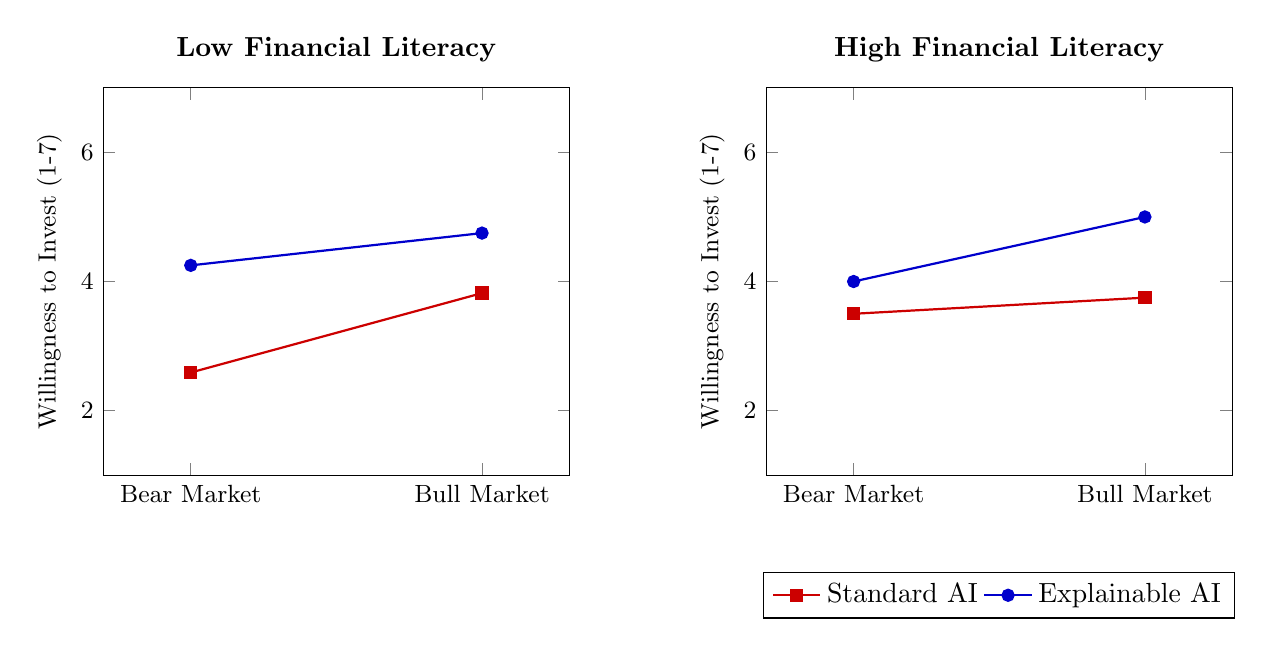
\begin{tikzpicture}
\begin{groupplot}[
    group style={
        group size=2 by 1,
        horizontal sep=2.5cm
    },
    width=7.5cm,
    height=6.5cm,
    ymin=1, ymax=7,
    ylabel={Willingness to Invest (1-7)},
    xtick={0,1},
    xticklabels={Bear Market, Bull Market},
    enlarge x limits=0.3,
    legend style={at={(0.5,-0.25)}, anchor=north, legend columns=-1},
    tick label style={font=\small},
    label style={font=\small}
]
% PLOT 1: LOW FINANCIAL LITERACY
\nextgroupplot[title={\textbf{Low Financial Literacy}}]
% Standard AI: Bear(2.59), Bull(3.82)
\addplot[mark=square*, color=red!80!black, thick] coordinates {(0, 2.59) (1, 3.82)};
% Explainable AI: Bear(4.25), Bull(4.75)
\addplot[mark=*, color=blue!80!black, thick] coordinates {(0, 4.25) (1, 4.75)};

% PLOT 2: HIGH FINANCIAL LITERACY
\nextgroupplot[title={\textbf{High Financial Literacy}}]
% Standard AI: Bear(3.5), Bull(3.75)
\addplot[mark=square*, color=red!80!black, thick] coordinates {(0, 3.5) (1, 3.75)};
% Explainable AI: Bear(4.0), Bull(5.0)
\addplot[mark=*, color=blue!80!black, thick] coordinates {(0, 4.0) (1, 5.0)};
\legend{Standard AI, Explainable AI}
\end{groupplot}
\end{tikzpicture}
\caption{Three-way interaction effect on Willingness to Invest.}
\label{fig:interaction}
\end{figure}

% RIPRENDERE DA QUI

In particular, the largest increase associated with XAI is observed among low-financial-literacy participants in bear markets, whereas the effect is substantially smaller among highly financially literate participants. Conversely, under bull-market conditions, the advantage of XAI is more evident among highly financially literate participants.

To better characterize the significant three-way interaction, post-hoc pairwise comparisons were conducted using the ART procedure with Bonferroni-adjusted p-values. These comparisons identify the specific experimental conditions in which algorithmic transparency significantly affected willingness to invest.

Panel A compares Standard AI and XAI within each combination of market context and financial literacy. During bear markets, XAI significantly increased willingness to invest among low-financial-literacy participants ($p<.001$), whereas no significant difference emerged among highly financially literate participants ($p=1.000$). Under bull-market conditions, XAI significantly increased willingness to invest among highly financially literate participants ($p=.012$), while the corresponding effect among low-literacy participants was only marginal after Bonferroni correction ($p=.094$).

Panel B examines the effect of market context within each transparency condition. Among low-financial-literacy participants using Standard AI, willingness to invest was significantly lower in bear than in bull markets ($p<.001$). By contrast, this difference was no longer statistically significant under XAI ($p=1.000$), suggesting that explainability attenuated the negative impact of adverse market conditions for this subgroup.

Panel C reports additional cross-condition comparisons, confirming that the lowest willingness to invest was observed for low-literacy participants exposed to Standard AI during bear markets, whereas substantially higher scores were observed in the corresponding XAI conditions.

\clearpage

\begin{sidewaystable}[p]
\centering
\caption{Comprehensive Post-Hoc Pairwise Comparisons on Aligned Ranks}
\label{tab:artcon_full}
\begin{threeparttable}
\small
\fontfamily{cmr}\selectfont % Assicura il font standard accademico
\setlength{\tabcolsep}{18pt}   % Spazio orizzontale ampio tra le colonne
\renewcommand{\arraystretch}{1.3} % Interlinea aumentata per massima leggibilità

\begin{tabular}{llccccl}
\toprule
\textbf{Condition A} & \textbf{Condition B} & \textbf{Estimate} & \textbf{SE} & \textbf{\textit{t}(92)} & \textbf{\textit{p} (adj.)} & \textbf{Sig.} \\
\midrule

\multicolumn{7}{l}{\textbf{Panel A: The Mitigation of Algorithm Aversion via XAI within Market Contexts}} \\
Bear Market, XAI, High Literacy & Bear Market, Standard AI, High Literacy & 10.74 & 9.79 & 1.096 & 1.0000 & n.s. \\
Bear Market, XAI, Low Literacy  & Bear Market, Standard AI, Low Literacy  & 36.30 & 7.02 & 5.172 & $<.0001$ & *** \\
\cmidrule{1-7}
Bull Market, XAI, High Literacy & Bull Market, Standard AI, High Literacy & 35.87 & 9.79 & 3.663 & 0.0117 & * \\
Bull Market, XAI, Low Literacy  & Bull Market, Standard AI, Low Literacy  & 21.13 & 7.02 & 3.011 & 0.0942 & $\dagger$ \\

\midrule
\multicolumn{7}{l}{\textbf{Panel B: Asymmetric Market Shocks on Opaque vs. Explainable Algorithms}} \\
Bear Market, Standard AI, Low Literacy  & Bull Market, Standard AI, Low Literacy  & -48.43 & 7.02 & -6.899 & $<.0001$ & *** \\
Bear Market, Standard AI, High Literacy & Bull Market, Standard AI, High Literacy & -22.36 & 8.64 & -2.588 & 0.3137 & n.s. \\
\cmidrule{1-7}
Bear Market, XAI, Low Literacy  & Bull Market, XAI, Low Literacy  & -12.13 & 7.12 & -1.702 & 1.0000 & n.s. \\
Bear Market, XAI, High Literacy & Bull Market, XAI, High Literacy & -29.94 & 9.50 & -3.152 & 0.0612 & $\dagger$ \\

\midrule
\multicolumn{7}{l}{\textbf{Panel C: Cross-Condition Baseline Contrasts ( Opaque Crises vs. Transparent Growth )}} \\
Bear Market, Standard AI, Low Literacy  & Bull Market, XAI, Low Literacy  & -58.23 & 8.31 & -7.010 & $<.0001$ & *** \\
Bear Market, Standard AI, High Literacy & Bull Market, XAI, High Literacy & -40.68 & 9.79 & -4.155 & 0.0020 & ** \\
Bear Market, XAI, High Literacy         & Bear Market, Standard AI, Low Literacy  & 28.29 & 8.31 & 3.405 & 0.0275 & * \\
Bear Market, Standard AI, Low Literacy  & Bull Market, Standard AI, High Literacy & -27.29 & 6.91 & -3.949 & 0.0043 & ** \\
\bottomrule
\end{tabular}

\begin{tablenotes}
\footnotesize
\item \textit{Note.} Post-hoc contrasts computed on aligned ranks using the \texttt{art.con()} procedure \citep{wobbrock2011thealigned}. P-values are adjusted using the conservative Bonferroni correction over the family of 28 total tests. Estimate represents the difference in aligned rank scores between Condition A and Condition B.
\item $^{\dagger}p<.10$, $^{*}p<.05$, $^{**}p<.01$, $^{***}p<.001$.
\end{tablenotes}
\end{threeparttable}
\end{sidewaystable}

\clearpage

Overall, the post-hoc analyses indicate that the effect of XAI is conditional rather than universal. While transparency generally increases willingness to invest, its magnitude depends jointly on market conditions and investors' financial literacy. These findings provide partial support for the proposed hypotheses and reveal a more nuanced pattern than originally anticipated.

\section{Conclusion}

This preliminary study investigated whether Explainable AI (XAI) can mitigate algorithm aversion in investment decisions and whether this relationship depends on market conditions and investors' financial literacy. Overall, the findings provide partial support for the proposed hypotheses, revealing that the effect of algorithmic transparency is conditional rather than universal. While XAI generally increases willingness to invest, its impact varies substantially across market contexts and investor profiles. In particular, explainability appears to be most beneficial for individuals with lower financial literacy during bear markets, whereas in bull markets its benefits are more evident among highly financially literate investors.

These findings carry potentially relevant managerial implications. Rather than adopting a one-size-fits-all transparency strategy, investment funds may benefit from selectively providing intuitive and accessible explanations of their AI-driven investment processes, particularly during periods of heightened market uncertainty. Such targeted transparency could help reduce algorithm aversion, strengthen investor trust, and ultimately mitigate customer attrition during adverse market conditions.

Several limitations should be acknowledged. First, the study relies on a relatively small synthetic sample of Digital Twins generated through Large Language Models, making the results exploratory rather than conclusive. Second, financial literacy was operationalized through a median split, and additional individual characteristics were not incorporated into the present analysis. Future research should therefore replicate the experiment using a larger sample of real human participants, retain financial literacy as a continuous variable, incorporate relevant demographic and psychological covariates, and explore more comprehensive experimental designs, including multiple levels of algorithmic transparency, human-advisor benchmarks, and the mediating role of investors' emotional responses.

\clearpage

\bibliographystyle{apalike} % Forza lo stile APA
\bibliography{ref}    % Richiama il file references.bib


% ==========================================
% SEZIONE APPENDIX (Da mettere alla fine del documento, prima o dopo la bibliografia)
% ==========================================

\newpage
\appendix
\section{Experimental Simulation Details}

\subsection{Mental Trade-off Prompt and Vignette Randomization}
Each Digital Twin was exposed to a dynamically generated prompt containing their unique socio-demographic profile, followed by the randomized experimental stimuli (Market Context and Algorithm Transparency). The prompt was explicitly engineered to bypass the LLM's logical alignment and force a human-like behavioral response based on cognitive biases.

\begin{verbatim}
--- IDENTITY PROFILE ---
[Inserted from Twin-2K-500 dataset: persona_summary]
(Fin. Literacy: {fl}/7, Tech Savviness: {ts}/7).

--- SCENARIO ---
You are evaluating a new investment fund completely managed by an AI algorithm.
Current Environment: 
[Randomized: BULL MARKET: The economy is thriving, with consistent growth, high 
consumer confidence, and strong positive market trends over the last 12 months. 
OR 
BEAR MARKET: The economy is in a severe downturn, with high volatility, widespread 
financial losses, and significant uncertainty over the last 12 months.]

Algorithm Transparency: 
[Randomized:EXPLAINABLE AI (XAI): You have a dashboard showing
exact decision rationales, feature weights, and risk assessments.
OR
"STANDARD AI: You receive only standard performance KPIs. 
The internal decision logic is proprietary and completely hidden.]

--- TASK ---
You are a real human investor, subject to human emotions and cognitive biases. 
Do not act as a logical AI assistant.
1. Psychological Assessment: How do your personal biases, past financial fears, 
   and specific attitude towards new technologies react to this precise Market 
   Environment?
2. Decision: Given that specific emotional and cognitive state, how does this 
   Transparency Level impact your willingness to trust the fund?
\end{verbatim}

\newpage

\begin{verbatim}
3. Filter this decision entirely through your personal history and the 
   literacy/tech scores provided above.
Decide quickly: you must act before the market opens tomorrow.

--- SCALE ---
1 (Absolutely not willing to invest) to 7 (Extremely willing to invest).

--- OUTPUT ---
Respond ONLY with a single integer (1 to 7). Do not add ANY reasoning, 
explanations, or extra punctuation.
\end{verbatim}


\end{document}
